The individual predictions from the acoustic and the lexical model need to be combined to obtain a final, overall prediction.
Therefore, we fuse the predictions of the two models.
We implemented two different fusion approaches: 
The first approach is called \emph{Threshold Fusion}, the second \emph{Balance Fusion}.
The two fusion approaches and the evaluation will be presented in the remainder of this section.

\subsection{Threshold Fusion}
The main idea of the threshold fusion is the following: If the probability for the class \textsc{Period} from the acoustic model is over a certain threshold and the probability for the class \textsc{None} from the lexical model is below a certain threshold, we want to predict a period or a comma.
If the condition is satisfied, the probability of the class \textsc{Period} from the acoustic model is added to the probabilities of the classes \textsc{Period} and \textsc{Comma} from the lexical model.
The idea of the threshold fusion is shown in the Figure~\ref{fig:fusion_1}.
\begin{figure}[ht]
    \centering
    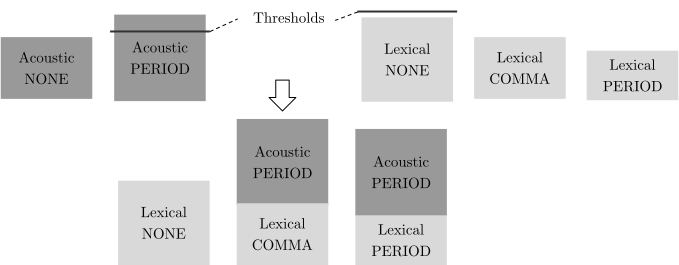
\includegraphics[width=0.7\textwidth]{img/fusion_1.pdf}
    \caption{Threshold Fusion: The probability of the class \textsc{Period} from the acoustic model is added to the probabilities of the classes \textsc{Period} and \textsc{Comma} from the lexical model, if the probability for the class \textsc{Period} from the acoustic model is over a certain threshold and the probability for the class \textsc{None} from the lexical model is below a certain threshold.}
    \label{fig:fusion_1}
\end{figure}
If the condition holds not, just the predictions of the lexical model are taken as final the predictions.
Thus, the threshold fusion trusts the lexical model more than the acoustic model.
The acoustic model is only taken into account, if the acoustic model is quite certain, that there should be a period, and the lexical model is not certain enough, that there should be no punctuation at all.
In the end, the class with the highest probability is chosen.
For the example in Figure~\ref{fig:fusion_1}, we would predict a comma. 

\subsection{Balance Fusion}
The balance fusion sums up weighted probabilities of both models.
Figure~\ref{fig:fusion_2} shows an example.
\begin{figure}[ht]
    \centering
    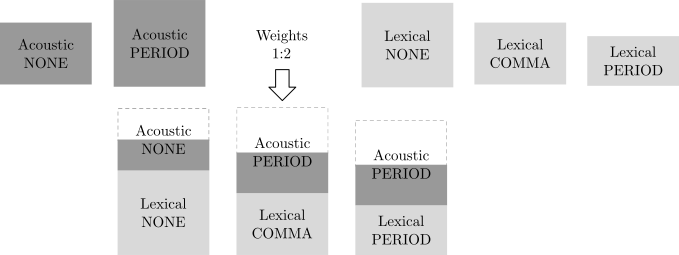
\includegraphics[width=0.7\textwidth]{img/fusion_2.pdf}
    \caption{Balance Fusion: Sum up the weighted probabilities of both models.}
    \label{fig:fusion_2}
\end{figure}
Using weights we can regulate, which model we trust more.
In the example shown in Figure~\ref{fig:fusion_2}, the lexical model is more important than the acoustic model. 
In the end, the class with the overall highest probability is chosen again.
So in the example, this would be the class \textsc{None}.

\subsection{Evaluation}
